In last section, we stated that information from ganglion cells is transmitted to the Lateral Geniculate Nucleus (part of the thalamus), where information is relayed and organized so that the cortex can interpret it. Studies on primates reveal that this organization means that the left visual field is sent to right hemisphere, and the right field to the left hemisphere (Figure~\ref{fig:vision:optic-chiasm})~\cite{thompson2000brain}. Inputs from ganglion cells with different receptive field sizes are separated into the magnocellular (for large fields) and parvocellular (for small fields) pathways.

\begin{figure}[h]
  \begin{center}
    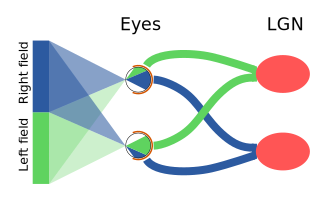
\includegraphics[width=0.5\textwidth]{visual-fields-lgn}
    \caption{Visual field mapping from the retina to the LGN.}
    \label{fig:vision:optic-chiasm}
  \end{center}
\end{figure}

It may seem like the LGN's only role is as a traffic controller, but it has centre-surround behaviour which could indicate that further compression is done in this section of the brain. Additionally, it receives connections from the cortex and the brainstem reticular formation, extra inputs could indicate a role in attention~\cite{eye-brain-vision-hubel1995}.

The region of the neocortex involved in visual processing is known as the \emph{visual cortex} and takes up around 30\% of the cortical area. Both hemispheres of the brain have symmetric areas involved in visual information processing. the portions that are involved in vision are thought to have a hierarchical organization, Figure~\ref{fig:vision:visual-cortex} shows a diagram of the areas of the cortex.

\begin{figure}[h]
  \begin{center}
    \begin{subfigure}[b]{0.65\textwidth}
      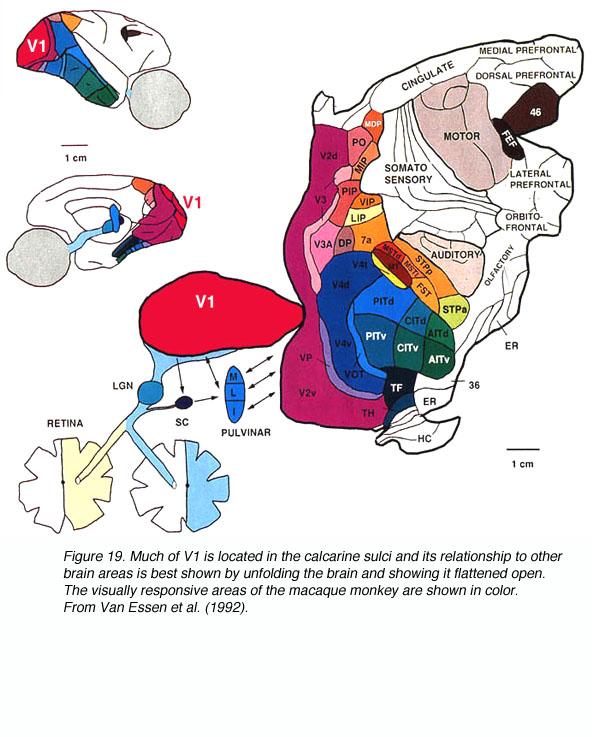
\includegraphics[width=\textwidth]{Visual-Cortex1}
      \caption{Areas related to vision~\cite{webvision-images}.}
      \label{fig:vision:visual-cortex}
    \end{subfigure}
    \begin{subfigure}[b]{0.34\textwidth}
      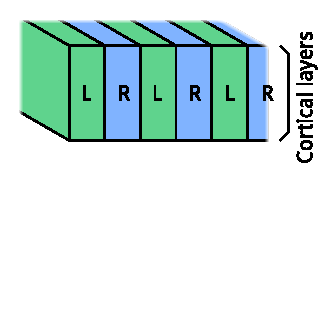
\includegraphics[width=\textwidth]{cortex-LR}
      \caption{Columnar organization.}
      \label{fig:vision:visual-cortex-LR}
    \end{subfigure}
    \caption{Diagrams of the visual cortex. Left, flattened surface of the Macaque brain. Right, inputs from left and right eyes are interleaved in the cortex. }
  \end{center}
\end{figure}

Fibres running from LGN lead to the primary visual cortex (V1), where there is a spatial correspondence between the retina/LGN and V1. The foveal region of the retina takes a large part of the area of V1, most likely to account for high resolution of the fovea. In V1, connections are organized so that inputs from the left eye are interleaved with the ones coming from the right eye, this makes cells in one slab (Figure~\ref{fig:vision:visual-cortex-LR}) react stronger to the dominant eye. Neurons in V1 can discriminate the spatial orientation, frequency, and colour of their input; and, in that sense, it might be seen as an edge detector. The output of the primary visual cortex then follows two paths, the dorsal (upper) and the ventral (lower) stream. The dorsal stream has selectiveness for shapes and direction, and the ventral adds colour discrimination~\cite{thompson2000brain}. This is, to some extent, expected because the dorsal stream is fed by the magnocellular pathway of LGN, which should have representations of broad shapes. On the other hand, the ventral stream receives information from the parvocellular pathway, that should have more colour and higher resolution information\cite{webvision}.

The next stage of the visual processing pipeline is known as V2, most of its input comes from V1 and its output goes to V3, V4 and V5. There are also feedback connections to V1. It is thought to respond to more complex shapes than V1. 

The exact area that V3 occupies is still a matter of debate as is its function, but the literature suggests that it could have a full representation of the shapes and that it has some role in motion selectivity in V5. 

Visual area V4 receives most of its input from V2 and presents 
discrimination for spatial orientation and frequency and also to colour. It is thought to have a representation of features more complex than V1 or V2, but not as much as full faces. The visual section of the middle temporal (MT) area is known as V5. This region is thought to have specially good response to motion, depth perception and control of eye movements. 

The next area in the ventral stream (V6) is thought to be able to distinguish shapes (e.g. circles from squares) and a preference for almost flat portions of the visual field. Further, the visual temporal area (TE) strongly responds to specific complex shapes (e.g. faces or  hands)\cite{eye-brain-vision-hubel1995,thompson2000brain}.
